\documentclass[11pt, oneside,margin=1in]{article}   	% use "amsart" instead of "article" for AMSLaTeX format

\usepackage{geometry}
 \geometry{
 a4paper,
 total={170mm,257mm},
 top=20mm,
 }               		% ... or a4paper or a5paper or ... 
%\geometry{landscape}                		% Activate for for rotated page geometry
%\usepackage[parfill]{parskip}    		% Activate to begin paragraphs with an empty line rather than an indent
\usepackage{graphicx}				% Use pdf, png, jpg, or eps§ with pdflatex; use eps in DVI mode
								% TeX will automatically convert eps --> pdf in pdflatex		
\usepackage{amssymb}
\usepackage{CJKutf8}
\pagestyle{empty}
\newcommand{\chuhao}{\fontsize{14bp}{\baselineskip}}
\linespread{1.2}
\begin{document}
\begin{CJK}{UTF8}{bkai}
%\section{}
%\subsection{}


\chuhao尊敬的<<<name>>>,
\par
您好,您繳納的200元會費已確認收到,歡迎您成為香港新疆聯誼會的會員!您的會員號為<<<id>>>,會員資格有效期至<<<date>>>。

\section*{\chuhao作為會員,您享有以下福利}
\begin{description}
\item每年一到兩次會員免費活動。
\item每年一到兩次會員專屬活動。
\item所有公開報名的活動,費用八五折。
\end{description}


香港新疆聯誼會處於創建時期,我們會持續尋求更多資源,為會員帶來更好的福利,也希望您能夠推廣聯誼會,一起把組織做好。如果您有好的建議和資源,歡迎郵件聯系我們。


\section*{\chuhao香港新疆聯誼會的主要信息媒介和聯系方式如下}
\begin{center}
\begin{description}
\item官方主頁: www.hkaxj.com
\item郵箱: contact@hkaxj.com
\item微信:\center 
\includegraphics[width=1.5in]{./res/qr.jpg} 
\end{description}
\end{center}
\section*{\chuhao香港新疆聯誼會的每次活動都會以郵件形式向您通知,活動頻率約為每月一次,請您關注注冊郵箱。}
\center
\begin{tabular}{ l c r r }
 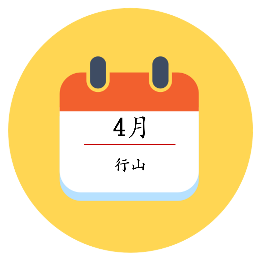
\includegraphics[width=1.2in]{res/4.png} &  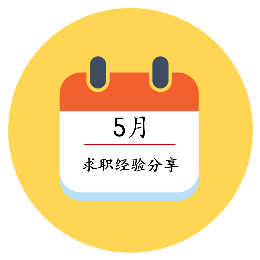
\includegraphics[width=1.2in]{res/5.png}  &  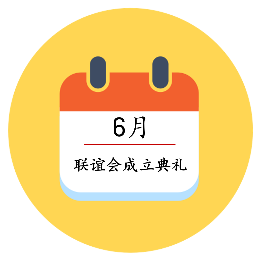
\includegraphics[width=1.2in]{res/6.png}  &  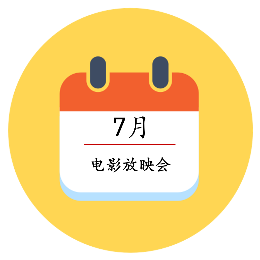
\includegraphics[width=1.2in]{res/7.png} \\
 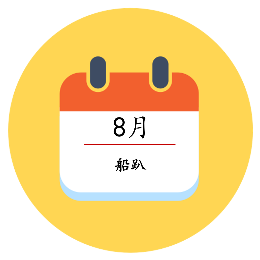
\includegraphics[width=1.2in]{res/8.png} &  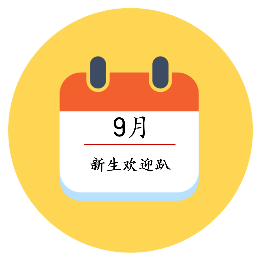
\includegraphics[width=1.2in]{res/9.png} &  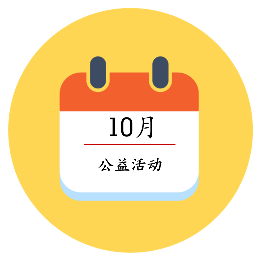
\includegraphics[width=1.2in]{res/10.png} &  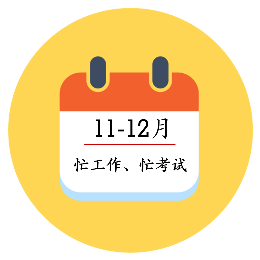
\includegraphics[width=1.2in]{res/11.png} \\
\end{tabular}

\end{CJK}
\end{document}  